\documentclass[a4paper, 10pt]{scrartcl}\usepackage[]{graphicx}\usepackage[]{color}
%% maxwidth is the original width if it is less than linewidth
%% otherwise use linewidth (to make sure the graphics do not exceed the margin)
\makeatletter
\def\maxwidth{ %
  \ifdim\Gin@nat@width>\linewidth
    \linewidth
  \else
    \Gin@nat@width
  \fi
}
\makeatother

\definecolor{fgcolor}{rgb}{0.345, 0.345, 0.345}
\newcommand{\hlnum}[1]{\textcolor[rgb]{0.686,0.059,0.569}{#1}}%
\newcommand{\hlstr}[1]{\textcolor[rgb]{0.192,0.494,0.8}{#1}}%
\newcommand{\hlcom}[1]{\textcolor[rgb]{0.678,0.584,0.686}{\textit{#1}}}%
\newcommand{\hlopt}[1]{\textcolor[rgb]{0,0,0}{#1}}%
\newcommand{\hlstd}[1]{\textcolor[rgb]{0.345,0.345,0.345}{#1}}%
\newcommand{\hlkwa}[1]{\textcolor[rgb]{0.161,0.373,0.58}{\textbf{#1}}}%
\newcommand{\hlkwb}[1]{\textcolor[rgb]{0.69,0.353,0.396}{#1}}%
\newcommand{\hlkwc}[1]{\textcolor[rgb]{0.333,0.667,0.333}{#1}}%
\newcommand{\hlkwd}[1]{\textcolor[rgb]{0.737,0.353,0.396}{\textbf{#1}}}%
\let\hlipl\hlkwb

\usepackage{framed}
\makeatletter
\newenvironment{kframe}{%
 \def\at@end@of@kframe{}%
 \ifinner\ifhmode%
  \def\at@end@of@kframe{\end{minipage}}%
  \begin{minipage}{\columnwidth}%
 \fi\fi%
 \def\FrameCommand##1{\hskip\@totalleftmargin \hskip-\fboxsep
 \colorbox{shadecolor}{##1}\hskip-\fboxsep
     % There is no \\@totalrightmargin, so:
     \hskip-\linewidth \hskip-\@totalleftmargin \hskip\columnwidth}%
 \MakeFramed {\advance\hsize-\width
   \@totalleftmargin\z@ \linewidth\hsize
   \@setminipage}}%
 {\par\unskip\endMakeFramed%
 \at@end@of@kframe}
\makeatother

\definecolor{shadecolor}{rgb}{.97, .97, .97}
\definecolor{messagecolor}{rgb}{0, 0, 0}
\definecolor{warningcolor}{rgb}{1, 0, 1}
\definecolor{errorcolor}{rgb}{1, 0, 0}
\newenvironment{knitrout}{}{} % an empty environment to be redefined in TeX

\usepackage{alltt}
\usepackage[margin=2.5cm
  %,showframe% <- only to show the page layout
]{geometry}

\usepackage{float}
\usepackage{graphicx}

\usepackage{amsmath}
%\renewcommand{\familydefault}{\sfdefault}

\usepackage{hyperref}
\hypersetup{
    colorlinks,
    citecolor=black,
    filecolor=black,
    linkcolor=blue,
    urlcolor=black
}

\title{Supplementary information: Among-species heterogeneity in sample size does not bias the estimation of synchrony}
\date{\today}
\author{Timoth\'ee Bonnet}
\IfFileExists{upquote.sty}{\usepackage{upquote}}{}
\begin{document}

\maketitle

\tableofcontents

\clearpage

\section{Goal and rationale}
The primary goal of this appendix is to test the idea that among-species heterogeneity in sample size might bias the estimation of synchrony among species. The verbal argument behind this concern is that the time-dynamic of the most common species might "spill over" the estimation of the time-dynamic common to all species. 
A suggested solution to this problem has been not to model synchrony explicitly, so that the model does not contain an across-species time-dynamic, but instead to estimate species-specific time dynamics independently, and reconstruct the synchrony a posteriori. Technically, this would be done by fitting a species-by-time random interaction without fitting the main random effect of time (but fitting the main random effect of species).

However, theory suggest that mixed models are generally able to handle unbalanced data, and that the estimation of synchrony should not be biased by unequal sample sizes.
Moreover, theory also suggests that the "solution" of not modeling synchrony explicitly and reconstructed it a posteriori from model prediction is flawed, and will generally lead to  under-estimation.

Here, we test that these two expectations hold for the special case of mixed mark-recapture models used in the main text, and that the results presented in the main text do not suffer from a bias due to unequal sample size among species.
To this end, we first multi-species mark-recapture data with synchrony among species or with no synchrony among species. We use the same sample size per year and per species as in the real data, but halved, in order to speed up modeling.  
We then analyse the simulated data either with a model that explicitly contain synchrony, or with a model that does not contain explicit synchrony but only allow for its reconstruction from species-specific estimates.

We first show that when sychrony is present in simulated data, a model explicitly modeling synchrony can recover it. We then show that on the same data, a model that does not explicitly model synchrony, but instead makes it estimation possible a posteriori, fails to estimate synchrony.
Finally, we show that the first model (explicitly modeling synchrony) does not detect synchrony if none is simulated in the data.

\section{Load packages and data}
We need \texttt{R2jags} to communicate with \texttt{JAGS}.
We use \texttt{reshape} to convert a matrix into a data frame.
We use \texttt{lme4} for variance partitioning.
We also load the real sample sizes per species per year.
\begin{knitrout}
\definecolor{shadecolor}{rgb}{0.969, 0.969, 0.969}\color{fgcolor}\begin{kframe}
\begin{alltt}
\hlkwd{setwd}\hlstd{(}\hlkwc{dir} \hlstd{=} \hlstr{"~/Documents/GitHub/penguinteam/SimulsForPubli/"}\hlstd{)}
\hlkwd{library}\hlstd{(R2jags)}
\end{alltt}


{\ttfamily\noindent\itshape\color{messagecolor}{\#\# Loading required package: rjags}}

{\ttfamily\noindent\itshape\color{messagecolor}{\#\# Loading required package: coda}}

{\ttfamily\noindent\itshape\color{messagecolor}{\#\# Linked to JAGS 4.2.0}}

{\ttfamily\noindent\itshape\color{messagecolor}{\#\# Loaded modules: basemod,bugs}}

{\ttfamily\noindent\itshape\color{messagecolor}{\#\# \\\#\# Attaching package: 'R2jags'}}

{\ttfamily\noindent\itshape\color{messagecolor}{\#\# The following object is masked from 'package:coda':\\\#\# \\\#\#\ \ \ \  traceplot}}\begin{alltt}
\hlkwd{library}\hlstd{(reshape)}
\hlkwd{library}\hlstd{(lme4)}
\end{alltt}


{\ttfamily\noindent\itshape\color{messagecolor}{\#\# Loading required package: Matrix}}

{\ttfamily\noindent\itshape\color{messagecolor}{\#\# \\\#\# Attaching package: 'Matrix'}}

{\ttfamily\noindent\itshape\color{messagecolor}{\#\# The following object is masked from 'package:reshape':\\\#\# \\\#\#\ \ \ \  expand}}\begin{alltt}
\hlstd{SpNumbers} \hlkwb{<-} \hlkwd{read.table}\hlstd{(}\hlkwc{file} \hlstd{=} \hlstr{"SpNumbers.txt"}\hlstd{,} \hlkwc{header}\hlstd{=}\hlnum{TRUE}\hlstd{)}
\hlstd{SpNumbers} \hlkwb{<-} \hlstd{SpNumbers[,}\hlopt{-}\hlnum{1}\hlstd{]}
\end{alltt}
\end{kframe}
\end{knitrout}

\section{Strong synchrony}

\subsection{Data simulation}

We use an additive model to simulate data, so that the effect of time is the same for all species, leading to strong (virtually perfect) synchrony. 

\begin{knitrout}
\definecolor{shadecolor}{rgb}{0.969, 0.969, 0.969}\color{fgcolor}\begin{kframe}
\begin{alltt}
\hlstd{n.occasions} \hlkwb{<-} \hlkwd{ncol}\hlstd{(SpNumbers)}  \hlcom{# Number of capture occasions}
\hlstd{meanphi} \hlkwb{<-} \hlnum{0} \hlcom{#logit intercept survival (i.e 0.5 on survival scale)}
\hlstd{effect_Occasions}\hlkwb{<-}\hlkwd{c}\hlstd{(}\hlnum{0}\hlstd{,}\hlkwd{rnorm}\hlstd{(}\hlkwc{n} \hlstd{= n.occasions}\hlopt{-}\hlnum{2}\hlstd{,}\hlkwc{mean} \hlstd{=} \hlnum{0}\hlstd{,}\hlkwc{sd} \hlstd{=} \hlnum{0.5}\hlstd{))}\hlcom{#time effect}

\hlstd{n.sp} \hlkwb{<-} \hlkwd{nrow}\hlstd{(SpNumbers)}
\hlstd{effect_Sp}\hlkwb{<-}\hlkwd{c}\hlstd{(}\hlnum{0}\hlstd{,}\hlkwd{rnorm}\hlstd{(}\hlkwc{n} \hlstd{= n.sp}\hlopt{-}\hlnum{1}\hlstd{,}\hlkwc{mean}\hlstd{=}\hlnum{0}\hlstd{,}\hlkwc{sd}\hlstd{=}\hlnum{1}\hlstd{))}


\hlcom{#marked <- round(100*(1:n.sp)^-2)   # Annual number of newly marked individuals}
\hlstd{p} \hlkwb{<-} \hlkwd{rep}\hlstd{(}\hlnum{0.4}\hlstd{, n.occasions}\hlopt{-}\hlnum{1}\hlstd{)}\hlcom{#constant recapture probability}

\hlcom{# Define matrices with survival and recapture probabilities}
\hlstd{PHI} \hlkwb{<-} \hlkwd{matrix}\hlstd{(} \hlkwc{data} \hlstd{=} \hlnum{NA}\hlstd{,} \hlkwc{ncol} \hlstd{= n.occasions}\hlopt{-}\hlnum{1}\hlstd{,} \hlkwc{nrow} \hlstd{=} \hlkwd{sum}\hlstd{( SpNumbers) )}
\hlstd{SpTots} \hlkwb{<-} \hlkwd{rowSums}\hlstd{(SpNumbers)}
\hlstd{CumulTots} \hlkwb{<-} \hlkwd{c}\hlstd{(}\hlnum{0}\hlstd{,} \hlkwd{cumsum}\hlstd{(SpTots))}
\hlstd{sp_ind} \hlkwb{<-} \hlkwd{vector}\hlstd{(}\hlkwc{length} \hlstd{=} \hlkwd{sum}\hlstd{(SpTots))}
\hlkwa{for} \hlstd{(sp} \hlkwa{in} \hlnum{1}\hlopt{:}\hlstd{n.sp)}
\hlstd{\{}
  \hlstd{spe} \hlkwb{<-}  \hlstd{effect_Sp[sp]}
  \hlstd{sp_ind[(CumulTots[sp]}\hlopt{+}\hlnum{1}\hlstd{)}\hlopt{:}\hlstd{CumulTots[sp}\hlopt{+}\hlnum{1}\hlstd{]]} \hlkwb{<-} \hlstd{sp}
  \hlcom{#nind <- sum(SpNumbers[sp,])}
  \hlkwa{for} \hlstd{(occ} \hlkwa{in} \hlnum{1}\hlopt{:}\hlstd{(n.occasions}\hlopt{-}\hlnum{1}\hlstd{))}
  \hlstd{\{}
    \hlstd{oce} \hlkwb{<-} \hlstd{effect_Occasions[occ]}
    \hlstd{PHI[(CumulTots[sp]}\hlopt{+}\hlnum{1}\hlstd{)}\hlopt{:}\hlstd{CumulTots[sp}\hlopt{+}\hlnum{1}\hlstd{],occ]} \hlkwb{<-} \hlnum{1}\hlopt{/}\hlstd{(}\hlnum{1}\hlopt{+}\hlkwd{exp}\hlstd{(}\hlopt{-}\hlstd{( meanphi} \hlopt{+} \hlstd{oce} \hlopt{+} \hlstd{spe) ) )}
  \hlstd{\}}

\hlstd{\}}

\hlstd{P} \hlkwb{<-} \hlkwd{matrix}\hlstd{(p,} \hlkwc{ncol} \hlstd{= n.occasions}\hlopt{-}\hlnum{1}\hlstd{,} \hlkwc{nrow} \hlstd{=} \hlkwd{sum}\hlstd{(SpTots))}
\end{alltt}
\end{kframe}
\end{knitrout}

\begin{knitrout}
\definecolor{shadecolor}{rgb}{0.969, 0.969, 0.969}\color{fgcolor}\begin{kframe}
\begin{alltt}
\hlcom{# Define function to simulate a capture-history (CH) matrix}
\hlstd{simul.cjs} \hlkwb{<-} \hlkwa{function}\hlstd{(}\hlkwc{PHI}\hlstd{,} \hlkwc{P}\hlstd{,} \hlkwc{SpTots}\hlstd{)\{}
  \hlstd{n.occasions} \hlkwb{<-} \hlkwd{dim}\hlstd{(PHI)[}\hlnum{2}\hlstd{]} \hlopt{+} \hlnum{1}
  \hlstd{CH} \hlkwb{<-} \hlkwd{matrix}\hlstd{(}\hlnum{0}\hlstd{,} \hlkwc{ncol} \hlstd{= n.occasions,} \hlkwc{nrow} \hlstd{=} \hlkwd{sum}\hlstd{(SpTots))}
  \hlstd{mark.occ} \hlkwb{<-} \hlkwd{rep}\hlstd{(}\hlnum{1}\hlopt{:}\hlkwd{length}\hlstd{(SpTots), SpTots[}\hlnum{1}\hlopt{:}\hlkwd{length}\hlstd{(SpTots)])}  \hlcom{# Define a vector with the occasion of marking}

  \hlkwa{for} \hlstd{(i} \hlkwa{in} \hlnum{1}\hlopt{:}\hlkwd{sum}\hlstd{(SpTots))\{}\hlcom{# Fill the CH matrix}
    \hlstd{CH[i, mark.occ[i]]} \hlkwb{<-} \hlnum{1}       \hlcom{# Write an 1 at the release occasion}
    \hlkwa{if} \hlstd{(mark.occ[i]}\hlopt{==}\hlstd{n.occasions)} \hlkwa{next}
    \hlkwa{for} \hlstd{(t} \hlkwa{in} \hlstd{(mark.occ[i]}\hlopt{+}\hlnum{1}\hlstd{)}\hlopt{:}\hlstd{n.occasions)\{}
      \hlcom{# Bernoulli trial: does individual survive occasion?}
      \hlstd{sur} \hlkwb{<-} \hlkwd{rbinom}\hlstd{(}\hlnum{1}\hlstd{,} \hlnum{1}\hlstd{, PHI[i,t}\hlopt{-}\hlnum{1}\hlstd{])}
      \hlkwa{if} \hlstd{(sur}\hlopt{==}\hlnum{0}\hlstd{)} \hlkwa{break}         \hlcom{# If dead, move to next individual }

      \hlstd{rp} \hlkwb{<-} \hlkwd{rbinom}\hlstd{(}\hlnum{1}\hlstd{,} \hlnum{1}\hlstd{, P[i,t}\hlopt{-}\hlnum{1}\hlstd{])}\hlcom{# Bernoulli trial: is individual recaptured? }
      \hlkwa{if} \hlstd{(rp}\hlopt{==}\hlnum{1}\hlstd{) CH[i,t]} \hlkwb{<-} \hlnum{1}
    \hlstd{\}} \hlcom{#t}
  \hlstd{\}} \hlcom{#i}
  \hlkwd{return}\hlstd{(CH)}
\hlstd{\}}
\end{alltt}
\end{kframe}
\end{knitrout}

\begin{knitrout}
\definecolor{shadecolor}{rgb}{0.969, 0.969, 0.969}\color{fgcolor}\begin{kframe}
\begin{alltt}
\hlcom{# Execute function}
\hlstd{CH} \hlkwb{<-} \hlkwd{simul.cjs}\hlstd{(PHI, P, SpTots)}

\hlcom{# Create vector with occasion of marking}
\hlstd{get.first} \hlkwb{<-} \hlkwa{function}\hlstd{(}\hlkwc{x}\hlstd{)} \hlkwd{min}\hlstd{(}\hlkwd{which}\hlstd{(x}\hlopt{!=}\hlnum{0}\hlstd{))}
\hlstd{f} \hlkwb{<-} \hlkwd{apply}\hlstd{(CH,} \hlnum{1}\hlstd{, get.first)}
\end{alltt}
\end{kframe}
\end{knitrout}


Functions to help fit MR models:

\begin{knitrout}
\definecolor{shadecolor}{rgb}{0.969, 0.969, 0.969}\color{fgcolor}\begin{kframe}
\begin{alltt}
\hlstd{known.state.cjs} \hlkwb{<-} \hlkwa{function}\hlstd{(}\hlkwc{ch}\hlstd{)\{}
  \hlstd{state} \hlkwb{<-} \hlstd{ch}
  \hlkwa{for} \hlstd{(i} \hlkwa{in} \hlnum{1}\hlopt{:}\hlkwd{dim}\hlstd{(ch)[}\hlnum{1}\hlstd{])\{}
    \hlstd{n1} \hlkwb{<-} \hlkwd{min}\hlstd{(}\hlkwd{which}\hlstd{(ch[i,]}\hlopt{==}\hlnum{1}\hlstd{))}
    \hlstd{n2} \hlkwb{<-} \hlkwd{max}\hlstd{(}\hlkwd{which}\hlstd{(ch[i,]}\hlopt{==}\hlnum{1}\hlstd{))}
    \hlstd{state[i,n1}\hlopt{:}\hlstd{n2]} \hlkwb{<-} \hlnum{1}
    \hlstd{state[i,n1]} \hlkwb{<-} \hlnum{NA}
  \hlstd{\}}
  \hlstd{state[state}\hlopt{==}\hlnum{0}\hlstd{]} \hlkwb{<-} \hlnum{NA}
  \hlkwd{return}\hlstd{(state)}
\hlstd{\}}


\hlstd{cjs.init.z} \hlkwb{<-} \hlkwa{function}\hlstd{(}\hlkwc{ch}\hlstd{,}\hlkwc{f}\hlstd{)\{}
  \hlkwa{for} \hlstd{(i} \hlkwa{in} \hlnum{1}\hlopt{:}\hlkwd{dim}\hlstd{(ch)[}\hlnum{1}\hlstd{])\{}
    \hlkwa{if} \hlstd{(}\hlkwd{sum}\hlstd{(ch[i,])}\hlopt{==}\hlnum{1}\hlstd{)} \hlkwa{next}
    \hlstd{n2} \hlkwb{<-} \hlkwd{max}\hlstd{(}\hlkwd{which}\hlstd{(ch[i,]}\hlopt{==}\hlnum{1}\hlstd{))}
    \hlstd{ch[i,f[i]}\hlopt{:}\hlstd{n2]} \hlkwb{<-} \hlnum{NA}
  \hlstd{\}}
  \hlkwa{for} \hlstd{(i} \hlkwa{in} \hlnum{1}\hlopt{:}\hlkwd{dim}\hlstd{(ch)[}\hlnum{1}\hlstd{])\{}
    \hlstd{ch[i,}\hlnum{1}\hlopt{:}\hlstd{f[i]]} \hlkwb{<-} \hlnum{NA}
  \hlstd{\}}
  \hlkwd{return}\hlstd{(ch)}
\hlstd{\}}
\end{alltt}
\end{kframe}
\end{knitrout}


\subsection{Interaction model with explicit synchorny}
We now fit a model that try to estimate the synchrony on the data containing strong synchrony.

\begin{knitrout}
\definecolor{shadecolor}{rgb}{0.969, 0.969, 0.969}\color{fgcolor}\begin{kframe}
\begin{alltt}
\hlkwd{sink}\hlstd{(}\hlstr{"cjs-phi(spXt)p(.).jags"}\hlstd{)}
\hlkwd{cat}\hlstd{(}\hlstr{[1204 chars quoted with '"']}\hlstd{,}\hlkwc{fill} \hlstd{=} \hlnum{TRUE}\hlstd{)}
\hlkwd{sink}\hlstd{()}
\end{alltt}
\end{kframe}
\end{knitrout}



\begin{knitrout}
\definecolor{shadecolor}{rgb}{0.969, 0.969, 0.969}\color{fgcolor}\begin{kframe}
\begin{alltt}
\hlcom{# Bundle data}
\hlstd{jags.data} \hlkwb{<-} \hlkwd{list}\hlstd{(}\hlkwc{y} \hlstd{= CH,} \hlkwc{f} \hlstd{= f,} \hlkwc{nind} \hlstd{=} \hlkwd{dim}\hlstd{(CH)[}\hlnum{1}\hlstd{],}
                  \hlkwc{n.occasions} \hlstd{=} \hlkwd{dim}\hlstd{(CH)[}\hlnum{2}\hlstd{],}
                  \hlkwc{z} \hlstd{=} \hlkwd{known.state.cjs}\hlstd{(CH),}
                  \hlkwc{sp_ind}\hlstd{=sp_ind,} \hlkwc{n.sp}\hlstd{=n.sp)}

\hlcom{#### Initial values####}
\hlcom{#interaction init}

\hlstd{beta.tXsp_ini}\hlkwb{<-}\hlkwa{function}\hlstd{()}
\hlstd{\{beta.tXsp}\hlkwb{<-}\hlkwd{matrix}\hlstd{(}\hlnum{NA}\hlstd{,}\hlkwc{nrow} \hlstd{= n.occasions}\hlopt{-}\hlnum{1}\hlstd{,}\hlkwc{ncol} \hlstd{= n.sp)}
\hlkwa{for} \hlstd{(i} \hlkwa{in} \hlnum{1}\hlopt{:}\hlstd{(n.occasions}\hlopt{-}\hlnum{1}\hlstd{))}
  \hlstd{\{}
    \hlkwa{for} \hlstd{(j} \hlkwa{in} \hlnum{1}\hlopt{:}\hlstd{n.sp)}
      \hlstd{\{}
        \hlstd{beta.tXsp[i,j]}\hlkwb{<-}\hlkwd{rnorm}\hlstd{(}\hlkwc{n} \hlstd{=} \hlnum{1}\hlstd{,}\hlkwc{mean} \hlstd{=} \hlnum{0}\hlstd{,}\hlkwc{sd} \hlstd{=} \hlnum{1}\hlstd{)}
      \hlstd{\}}
  \hlstd{\}}
\hlkwd{return}\hlstd{(beta.tXsp)}
\hlstd{\}}

\hlstd{inits} \hlkwb{<-} \hlkwa{function}\hlstd{()\{}\hlkwd{list}\hlstd{(}\hlkwc{z} \hlstd{=} \hlkwd{cjs.init.z}\hlstd{(CH, f),}
                \hlkwc{phi.mean} \hlstd{=} \hlkwd{runif}\hlstd{(}\hlnum{1}\hlstd{,} \hlnum{0}\hlstd{,} \hlnum{1}\hlstd{),} \hlkwc{p.mean} \hlstd{=} \hlkwd{runif}\hlstd{(}\hlnum{1}\hlstd{,} \hlnum{0}\hlstd{,} \hlnum{1}\hlstd{),}
                \hlkwc{beta.t}\hlstd{=}\hlkwd{c}\hlstd{(}\hlkwd{rnorm}\hlstd{(}\hlkwc{n} \hlstd{= n.occasions}\hlopt{-}\hlnum{1}\hlstd{,}\hlkwc{mean} \hlstd{=} \hlnum{0}\hlstd{,}\hlkwc{sd}\hlstd{=}\hlnum{1} \hlstd{) ),}
                \hlkwc{beta.sp}\hlstd{=}\hlkwd{c}\hlstd{(}\hlkwd{rnorm}\hlstd{(}\hlkwc{n} \hlstd{= n.sp,}\hlkwc{mean} \hlstd{=} \hlnum{0}\hlstd{,}\hlkwc{sd}\hlstd{=}\hlnum{1} \hlstd{) ),}
                \hlkwc{beta.tXsp}\hlstd{=} \hlkwd{beta.tXsp_ini}\hlstd{() )\}}

\hlcom{# Parameters monitored}
\hlstd{parameters} \hlkwb{<-} \hlkwd{c}\hlstd{(}\hlstr{"phi.mean"}\hlstd{,} \hlstr{"p.mean"}\hlstd{,}
                \hlstr{"beta.t"}\hlstd{,}\hlstr{"beta.sp"}\hlstd{,}
                \hlstr{"beta.tXsp"}\hlstd{,} \hlstr{"sigma.sp"}\hlstd{,}
                \hlstr{"sigma.t"}\hlstd{,} \hlstr{"sigma.tXsp"}\hlstd{)}

\hlcom{# MCMC settings}
\hlstd{ni} \hlkwb{<-} \hlnum{11000}
\hlstd{nt} \hlkwb{<-} \hlnum{10}
\hlstd{nb} \hlkwb{<-} \hlnum{1000}
\hlstd{nc} \hlkwb{<-} \hlnum{3}

\hlstd{cjs.interactionS} \hlkwb{<-} \hlkwd{jags}\hlstd{(jags.data, inits, parameters,}
                         \hlstr{"cjs-phi(spXt)p(.).jags"}\hlstd{,}
                        \hlkwc{n.chains} \hlstd{= nc,} \hlkwc{n.thin} \hlstd{= nt,}
                        \hlkwc{n.iter} \hlstd{= ni,} \hlkwc{n.burnin} \hlstd{= nb,}
                        \hlkwc{working.directory} \hlstd{=} \hlkwd{getwd}\hlstd{())}

\hlkwd{print}\hlstd{(cjs.interactionS,} \hlkwc{digits} \hlstd{=} \hlnum{3}\hlstd{)}
\end{alltt}
\end{kframe}
\end{knitrout}

\begin{knitrout}
\definecolor{shadecolor}{rgb}{0.969, 0.969, 0.969}\color{fgcolor}\begin{kframe}
\begin{alltt}
\hlkwd{load}\hlstd{(}\hlkwc{file} \hlstd{=} \hlstr{"ForCluster/cjs.interactionS_dataSynchro"}\hlstd{)}
\end{alltt}
\end{kframe}
\end{knitrout}

The synchrony is well recovered graphically:
\begin{knitrout}
\definecolor{shadecolor}{rgb}{0.969, 0.969, 0.969}\color{fgcolor}\begin{kframe}
\begin{alltt}
\hlcom{# Summarize posteriors}

\hlstd{predictions} \hlkwb{<-} \hlstd{cjs.interactionS}\hlopt{$}\hlstd{BUGSoutput}\hlopt{$}\hlstd{mean}\hlopt{$}\hlstd{beta.tXsp} \hlopt{+}
  \hlkwd{matrix}\hlstd{(cjs.interactionS}\hlopt{$}\hlstd{BUGSoutput}\hlopt{$}\hlstd{mean}\hlopt{$}\hlstd{beta.t,}
         \hlkwc{nrow} \hlstd{= n.occasions}\hlopt{-}\hlnum{1}\hlstd{,} \hlkwc{ncol} \hlstd{= n.sp,} \hlkwc{byrow} \hlstd{=} \hlnum{FALSE}\hlstd{)} \hlopt{+}
  \hlkwd{matrix}\hlstd{(cjs.interactionS}\hlopt{$}\hlstd{BUGSoutput}\hlopt{$}\hlstd{mean}\hlopt{$}\hlstd{beta.sp,}
         \hlkwc{nrow} \hlstd{= n.occasions}\hlopt{-}\hlnum{1}\hlstd{,} \hlkwc{ncol}\hlstd{=n.sp,} \hlkwc{byrow} \hlstd{=} \hlnum{TRUE}\hlstd{)}


\hlkwd{plot}\hlstd{(predictions[,}\hlnum{1}\hlstd{],} \hlkwc{type}\hlstd{=}\hlstr{"l"}\hlstd{,} \hlkwc{ylim}\hlstd{=}\hlkwd{c}\hlstd{(}\hlopt{-}\hlnum{3}\hlstd{,}\hlnum{3}\hlstd{),}
     \hlkwc{xlab}\hlstd{=}\hlstr{"year"}\hlstd{,} \hlkwc{main}\hlstd{=}\hlstr{"With year RE"}\hlstd{)}
\hlkwa{for}\hlstd{(i} \hlkwa{in} \hlnum{1}\hlopt{:}\hlstd{n.sp)}
\hlstd{\{}
  \hlkwd{lines}\hlstd{(predictions[,i])}
\hlstd{\}}
\end{alltt}
\end{kframe}
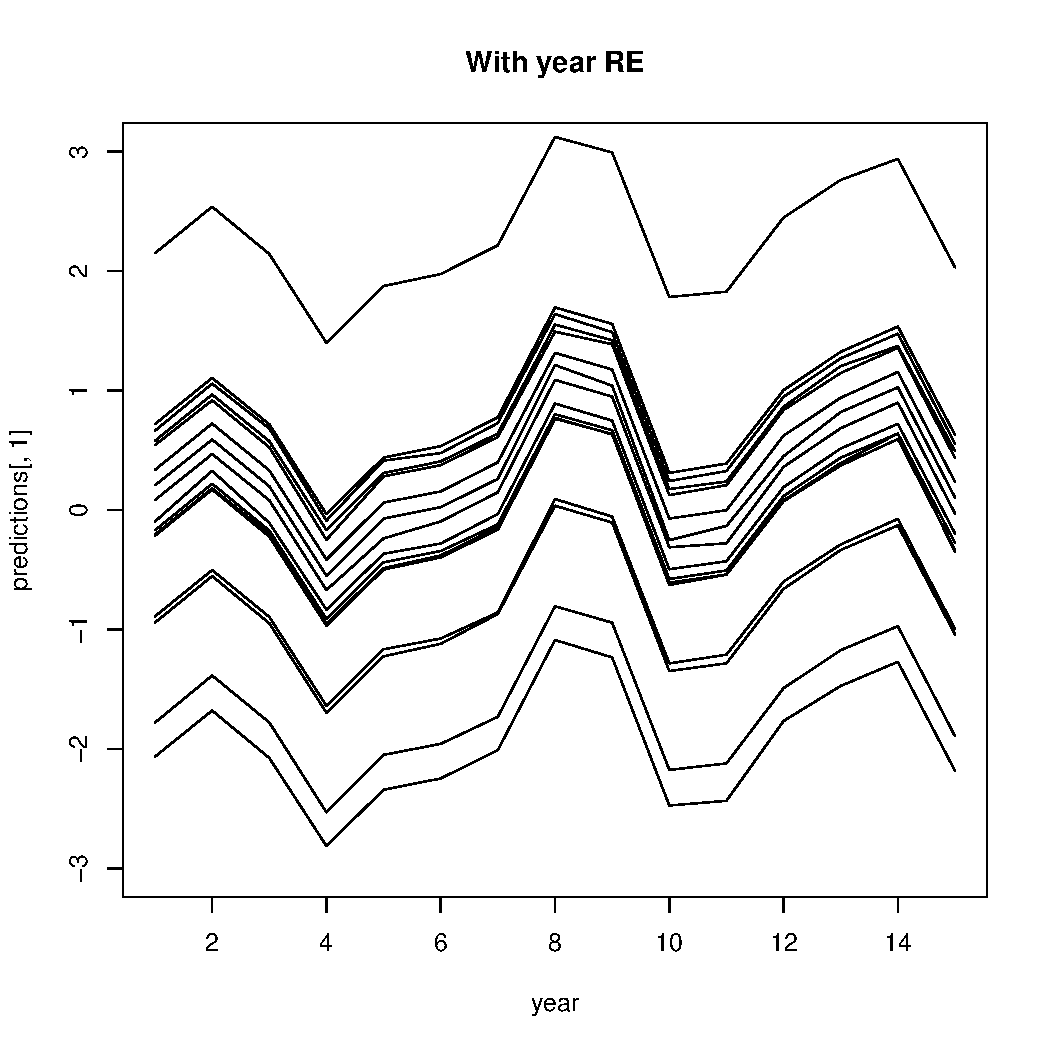
\includegraphics[width=\maxwidth]{figure/unnamed-chunk-9-1} 

\end{knitrout}

The intra-Class correlation is close to one, as revealed by the point estimate:
\begin{knitrout}
\definecolor{shadecolor}{rgb}{0.969, 0.969, 0.969}\color{fgcolor}\begin{kframe}
\begin{alltt}
\hlstd{(cjs.interactionS}\hlopt{$}\hlstd{BUGSoutput}\hlopt{$}\hlstd{mean}\hlopt{$}\hlstd{sigma.t}\hlopt{^}\hlnum{2}\hlstd{)}\hlopt{/}
  \hlstd{(cjs.interactionS}\hlopt{$}\hlstd{BUGSoutput}\hlopt{$}\hlstd{mean}\hlopt{$}\hlstd{sigma.tXsp}\hlopt{^}\hlnum{2}\hlopt{+}
     \hlstd{cjs.interactionS}\hlopt{$}\hlstd{BUGSoutput}\hlopt{$}\hlstd{mean}\hlopt{$}\hlstd{sigma.t}\hlopt{^}\hlnum{2}\hlstd{)}
\end{alltt}
\begin{verbatim}
## [1] 0.9717394
\end{verbatim}
\end{kframe}
\end{knitrout}

As well as the posterior distribution:
\begin{knitrout}
\definecolor{shadecolor}{rgb}{0.969, 0.969, 0.969}\color{fgcolor}\begin{kframe}
\begin{alltt}
\hlstd{iccpost} \hlkwb{<-} \hlkwd{vector}\hlstd{(}\hlkwc{length}\hlstd{=}\hlnum{1000}\hlstd{)}
\hlkwa{for} \hlstd{(ch} \hlkwa{in} \hlnum{1}\hlopt{:}\hlnum{1}\hlstd{)}
\hlstd{\{}
  \hlkwa{for} \hlstd{(itt} \hlkwa{in} \hlnum{1}\hlopt{:}\hlnum{1000}\hlstd{)}
  \hlstd{\{}
    \hlstd{iccpost[itt} \hlopt{+} \hlnum{1000}\hlopt{*}\hlstd{(ch}\hlopt{-}\hlnum{1}\hlstd{)]} \hlkwb{<-}
      \hlstd{cjs.interactionS}\hlopt{$}\hlstd{BUGSoutput}\hlopt{$}\hlstd{sims.array[itt, ch,}\hlstr{"sigma.t"}\hlstd{]}\hlopt{^}\hlnum{2} \hlopt{/}
      \hlstd{( cjs.interactionS}\hlopt{$}\hlstd{BUGSoutput}\hlopt{$}\hlstd{sims.array[itt, ch,}\hlstr{"sigma.t"}\hlstd{]}\hlopt{^}\hlnum{2} \hlopt{+}
          \hlstd{cjs.interactionS}\hlopt{$}\hlstd{BUGSoutput}\hlopt{$}\hlstd{sims.array[itt, ch,}\hlstr{"sigma.tXsp"}\hlstd{]}\hlopt{^}\hlnum{2}\hlstd{)}
  \hlstd{\}}
\hlstd{\}}


\hlstd{sdprior} \hlkwb{<-} \hlkwd{runif}\hlstd{(}\hlkwc{n} \hlstd{=} \hlnum{10000}\hlstd{,} \hlkwc{min} \hlstd{=} \hlnum{0}\hlstd{,} \hlkwc{max} \hlstd{=} \hlnum{10}\hlstd{)}
\hlstd{sdprior2} \hlkwb{<-} \hlstd{sdprior}

\hlstd{iccprior} \hlkwb{<-} \hlstd{(sdprior}\hlopt{^}\hlnum{2}\hlstd{)}\hlopt{/}\hlstd{(sdprior}\hlopt{^}\hlnum{2}\hlopt{+}\hlstd{sdprior2}\hlopt{^}\hlnum{2}\hlstd{)}

\hlkwd{traceplot}\hlstd{(}\hlkwd{as.mcmc}\hlstd{(iccpost),} \hlkwc{ylim}\hlstd{=}\hlkwd{c}\hlstd{(}\hlnum{0}\hlstd{,}\hlnum{1}\hlstd{))}
\end{alltt}
\end{kframe}
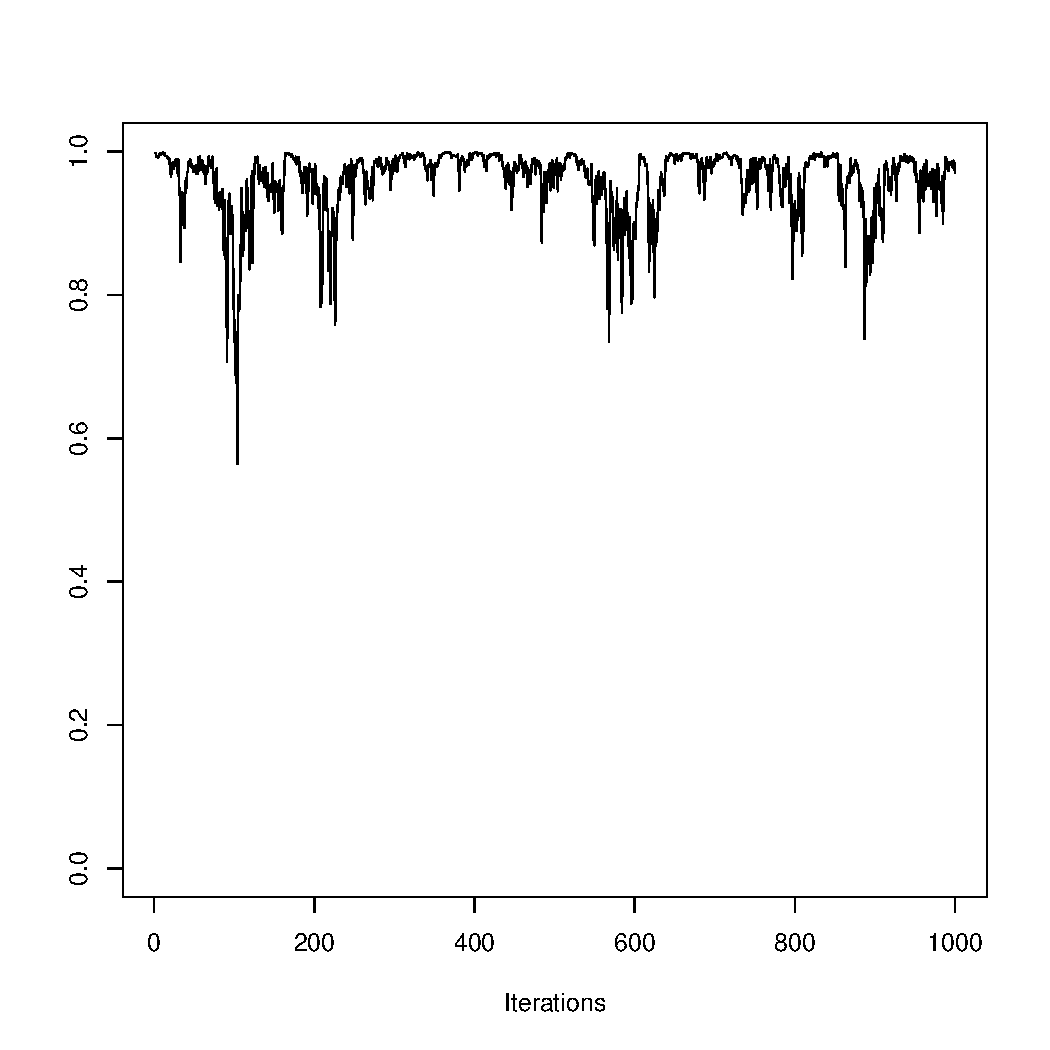
\includegraphics[width=\maxwidth]{figure/unnamed-chunk-11-1} 
\begin{kframe}\begin{alltt}
\hlkwd{plot}\hlstd{(}\hlkwd{density}\hlstd{(iccpost),} \hlkwc{xlim} \hlstd{=} \hlkwd{c}\hlstd{(}\hlnum{0}\hlstd{,}\hlnum{1}\hlstd{),} \hlkwc{lwd}\hlstd{=}\hlnum{5}\hlstd{,}
     \hlkwc{main}\hlstd{=}\hlstr{"Synchrony estimate with strong synchrony simulated (1)"}\hlstd{,}
     \hlkwc{xlab}\hlstd{=}\hlstr{"ICC"}\hlstd{,} \hlkwc{ylab}\hlstd{=}\hlstr{"Probability density"}\hlstd{)}

\hlkwd{lines}\hlstd{(}\hlkwd{density}\hlstd{(iccprior),} \hlkwc{lwd}\hlstd{=}\hlnum{3}\hlstd{,} \hlkwc{lty}\hlstd{=}\hlnum{2}\hlstd{,} \hlkwc{col}\hlstd{=}\hlstr{"gray"}\hlstd{)}
\end{alltt}
\end{kframe}
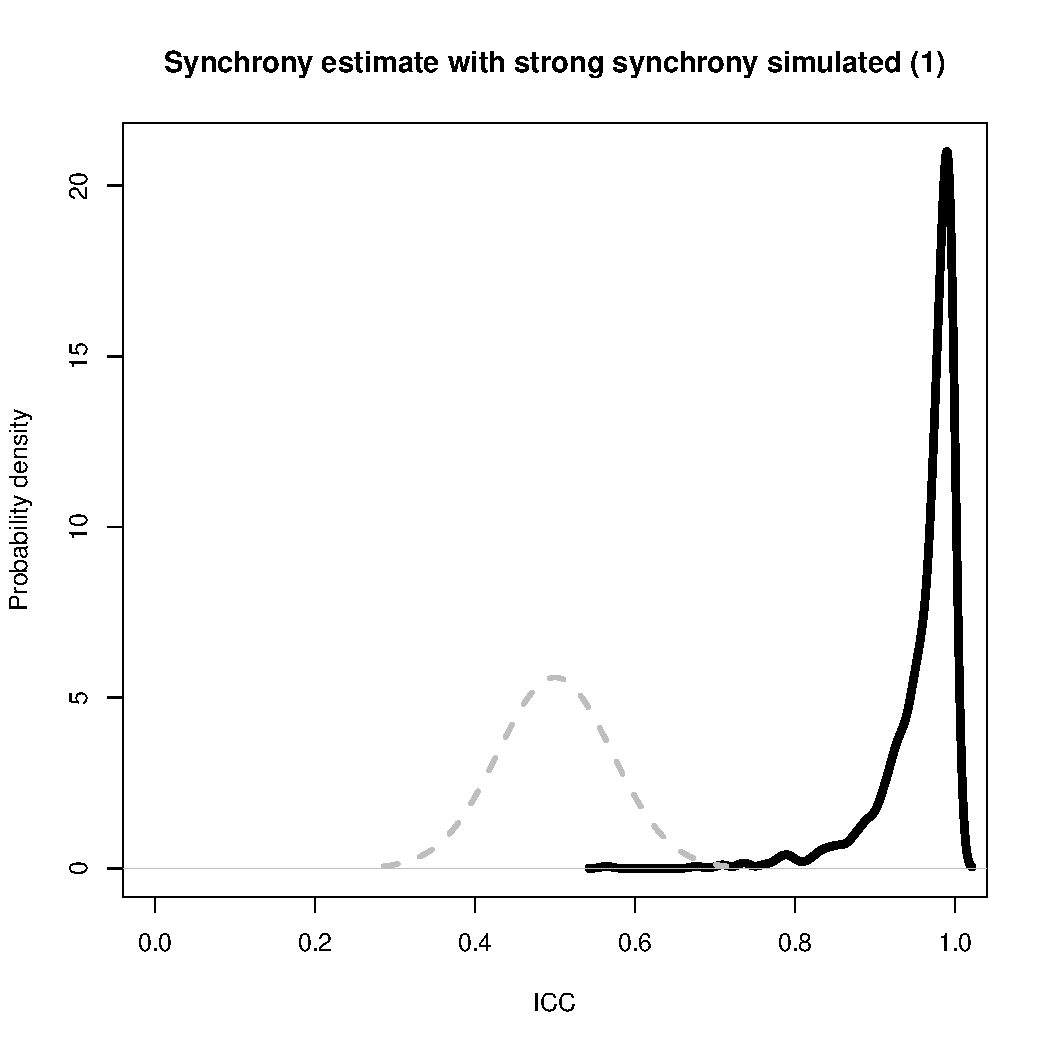
\includegraphics[width=\maxwidth]{figure/unnamed-chunk-11-2} 

\end{knitrout}

\subsection{Interactive model without explicit synchrony}
We analyse the same data, but this time using a model that does not explicitly contain synchrony.

\begin{knitrout}
\definecolor{shadecolor}{rgb}{0.969, 0.969, 0.969}\color{fgcolor}\begin{kframe}
\begin{alltt}
\hlkwd{sink}\hlstd{(}\hlstr{"cjs-phi(spXt_no_t)p(.).jags"}\hlstd{)}
\hlkwd{cat}\hlstd{(}\hlstr{[1060 chars quoted with '"']}\hlstd{,}\hlkwc{fill} \hlstd{=} \hlnum{TRUE}\hlstd{)}
\hlkwd{sink}\hlstd{()}
\end{alltt}
\end{kframe}
\end{knitrout}

\begin{knitrout}
\definecolor{shadecolor}{rgb}{0.969, 0.969, 0.969}\color{fgcolor}\begin{kframe}
\begin{alltt}
\hlcom{# Bundle data}
\hlstd{jags.data} \hlkwb{<-} \hlkwd{list}\hlstd{(}\hlkwc{y} \hlstd{= CH,} \hlkwc{f} \hlstd{= f,} \hlkwc{nind} \hlstd{=} \hlkwd{dim}\hlstd{(CH)[}\hlnum{1}\hlstd{],}
                  \hlkwc{n.occasions} \hlstd{=} \hlkwd{dim}\hlstd{(CH)[}\hlnum{2}\hlstd{],}
                  \hlkwc{z} \hlstd{=} \hlkwd{known.state.cjs}\hlstd{(CH),}
                  \hlkwc{sp_ind}\hlstd{=sp_ind,} \hlkwc{n.sp}\hlstd{=n.sp)}

\hlcom{#### Initial values####}
\hlcom{#interaction init}

\hlstd{beta.tXsp_ini}\hlkwb{<-}\hlkwa{function}\hlstd{()}
\hlstd{\{beta.tXsp}\hlkwb{<-}\hlkwd{matrix}\hlstd{(}\hlnum{NA}\hlstd{,}\hlkwc{nrow} \hlstd{= n.occasions}\hlopt{-}\hlnum{1}\hlstd{,}\hlkwc{ncol} \hlstd{= n.sp)}
\hlkwa{for} \hlstd{(i} \hlkwa{in} \hlnum{1}\hlopt{:}\hlstd{(n.occasions}\hlopt{-}\hlnum{1}\hlstd{))}
  \hlstd{\{}
    \hlkwa{for} \hlstd{(j} \hlkwa{in} \hlnum{1}\hlopt{:}\hlstd{n.sp)}
      \hlstd{\{}
        \hlstd{beta.tXsp[i,j]}\hlkwb{<-}\hlkwd{rnorm}\hlstd{(}\hlkwc{n} \hlstd{=} \hlnum{1}\hlstd{,}\hlkwc{mean} \hlstd{=} \hlnum{0}\hlstd{,}\hlkwc{sd} \hlstd{=} \hlnum{1}\hlstd{)}
      \hlstd{\}}
  \hlstd{\}}
\hlkwd{return}\hlstd{(beta.tXsp)}
\hlstd{\}}

\hlstd{inits} \hlkwb{<-} \hlkwa{function}\hlstd{()\{}\hlkwd{list}\hlstd{(}\hlkwc{z} \hlstd{=} \hlkwd{cjs.init.z}\hlstd{(CH, f),}
                  \hlkwc{phi.mean} \hlstd{=} \hlkwd{runif}\hlstd{(}\hlnum{1}\hlstd{,} \hlnum{0}\hlstd{,} \hlnum{1}\hlstd{),} \hlkwc{p.mean} \hlstd{=} \hlkwd{runif}\hlstd{(}\hlnum{1}\hlstd{,} \hlnum{0}\hlstd{,} \hlnum{1}\hlstd{),}
                  \hlkwc{beta.sp}\hlstd{=}\hlkwd{c}\hlstd{(}\hlkwd{rnorm}\hlstd{(}\hlkwc{n} \hlstd{= n.sp,}\hlkwc{mean} \hlstd{=} \hlnum{0}\hlstd{,}\hlkwc{sd}\hlstd{=}\hlnum{1} \hlstd{) ),}
                  \hlkwc{beta.tXsp}\hlstd{=} \hlkwd{beta.tXsp_ini}\hlstd{() )\}}

\hlcom{# Parameters monitored}
\hlstd{parameters} \hlkwb{<-} \hlkwd{c}\hlstd{(}\hlstr{"phi.mean"}\hlstd{,} \hlstr{"p.mean"}\hlstd{,}
                \hlstr{"beta.sp"}\hlstd{,}\hlstr{"beta.tXsp"}\hlstd{,}
                \hlstr{"sigma.sp"}\hlstd{,} \hlstr{"sigma.tXsp"}\hlstd{)}

\hlcom{# MCMC settings}
\hlstd{ni} \hlkwb{<-} \hlnum{11000}
\hlstd{nt} \hlkwb{<-} \hlnum{10}
\hlstd{nb} \hlkwb{<-} \hlnum{1000}
\hlstd{nc} \hlkwb{<-} \hlnum{3}

\hlstd{cjs.interactionNot} \hlkwb{<-} \hlkwd{jags}\hlstd{(jags.data, inits,}
                           \hlstd{parameters,} \hlstr{"cjs-phi(spXt_no_t)p(.).jags"}\hlstd{,}
                        \hlkwc{n.chains} \hlstd{= nc,} \hlkwc{n.thin} \hlstd{= nt,}
                        \hlkwc{n.iter} \hlstd{= ni,} \hlkwc{n.burnin} \hlstd{= nb,}
                        \hlkwc{working.directory} \hlstd{=} \hlkwd{getwd}\hlstd{())}

\hlkwd{print}\hlstd{(cjs.interactionNot,} \hlkwc{digits} \hlstd{=} \hlnum{3}\hlstd{)}
\end{alltt}
\end{kframe}
\end{knitrout}

\begin{knitrout}
\definecolor{shadecolor}{rgb}{0.969, 0.969, 0.969}\color{fgcolor}\begin{kframe}
\begin{alltt}
\hlkwd{load}\hlstd{(}\hlkwc{file} \hlstd{=} \hlstr{"ForCluster/cjs.interactionSNot_dataSynchro"}\hlstd{)}
\end{alltt}
\end{kframe}
\end{knitrout}

Graphically, much less synchrony is apparent:
\begin{knitrout}
\definecolor{shadecolor}{rgb}{0.969, 0.969, 0.969}\color{fgcolor}\begin{kframe}
\begin{alltt}
\hlstd{predictions} \hlkwb{<-}  \hlkwd{matrix}\hlstd{(cjs.interactionNot}\hlopt{$}\hlstd{BUGSoutput}\hlopt{$}\hlstd{mean}\hlopt{$}\hlstd{phi.mean,}
                       \hlkwc{nrow} \hlstd{= n.occasions}\hlopt{-}\hlnum{1}\hlstd{,} \hlkwc{ncol}\hlstd{=n.sp,} \hlkwc{byrow} \hlstd{=} \hlnum{TRUE}\hlstd{)} \hlopt{+}
      \hlstd{cjs.interactionNot}\hlopt{$}\hlstd{BUGSoutput}\hlopt{$}\hlstd{mean}\hlopt{$}\hlstd{beta.tXsp} \hlopt{+}
  \hlkwd{matrix}\hlstd{(cjs.interactionNot}\hlopt{$}\hlstd{BUGSoutput}\hlopt{$}\hlstd{mean}\hlopt{$}\hlstd{beta.sp,}
         \hlkwc{nrow} \hlstd{= n.occasions}\hlopt{-}\hlnum{1}\hlstd{,} \hlkwc{ncol}\hlstd{=n.sp,} \hlkwc{byrow} \hlstd{=} \hlnum{TRUE}\hlstd{)}


\hlkwd{plot}\hlstd{(predictions[,}\hlnum{1}\hlstd{],} \hlkwc{type}\hlstd{=}\hlstr{"l"}\hlstd{,} \hlkwc{ylim}\hlstd{=}\hlkwd{c}\hlstd{(}\hlopt{-}\hlnum{3}\hlstd{,}\hlnum{3}\hlstd{),} \hlkwc{xlab}\hlstd{=}\hlstr{"year"}\hlstd{,} \hlkwc{main}\hlstd{=}\hlstr{"With year RE"}\hlstd{)}
\hlkwa{for}\hlstd{(i} \hlkwa{in} \hlnum{1}\hlopt{:}\hlstd{n.sp)}
\hlstd{\{}
  \hlkwd{lines}\hlstd{(predictions[,i])}
\hlstd{\}}
\end{alltt}
\end{kframe}
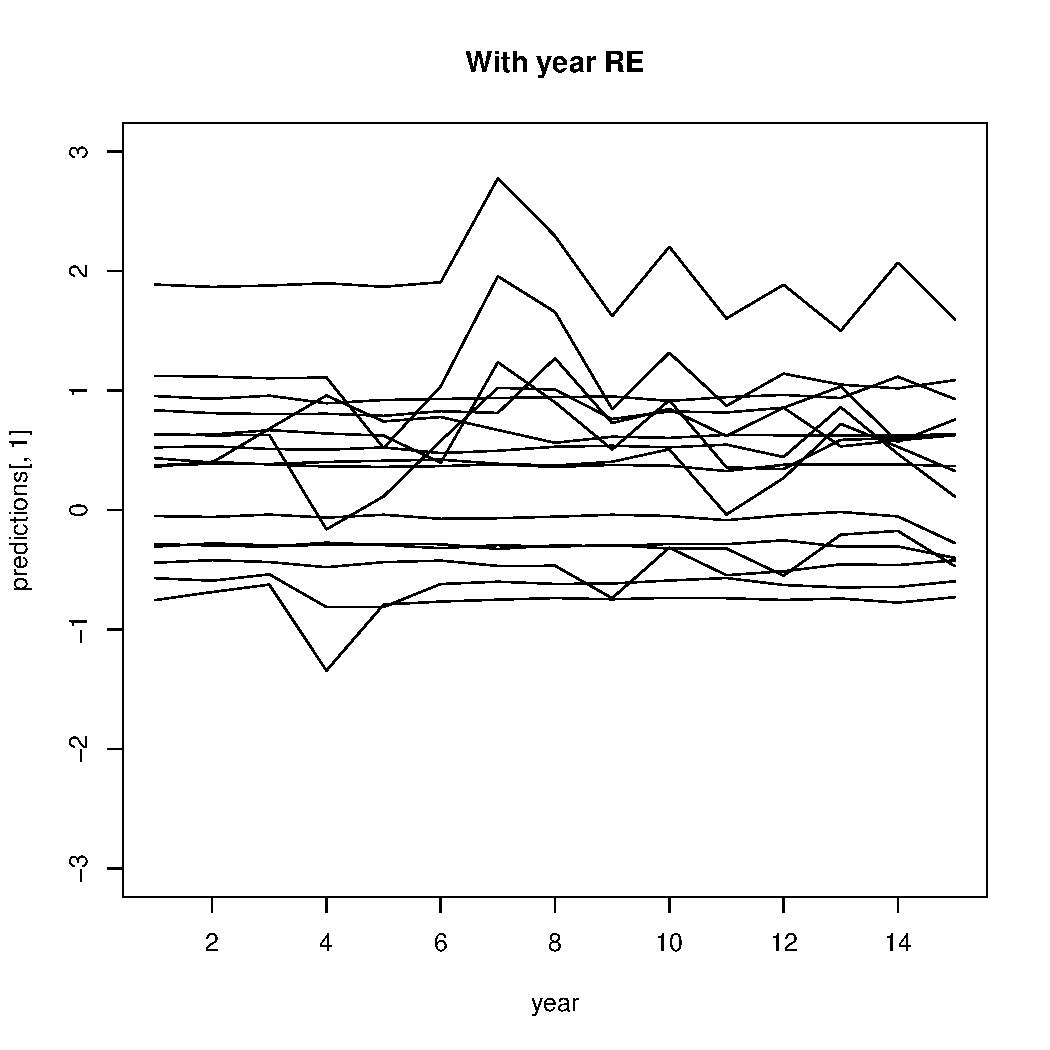
\includegraphics[width=\maxwidth]{figure/unnamed-chunk-15-1} 

\end{knitrout}

The intra class correlation (ratio of temporal variance common to all species over the total temporal variance) is weak and close to zero.
\begin{knitrout}
\definecolor{shadecolor}{rgb}{0.969, 0.969, 0.969}\color{fgcolor}\begin{kframe}
\begin{alltt}
\hlstd{meltedpredictions} \hlkwb{<-} \hlkwd{melt}\hlstd{(predictions)}
\hlkwd{summary}\hlstd{(}\hlkwd{aov}\hlstd{(}\hlkwc{formula} \hlstd{= value} \hlopt{~} \hlstd{X2} \hlopt{+} \hlstd{X1,} \hlkwc{data}\hlstd{=meltedpredictions))}
\end{alltt}
\begin{verbatim}
##              Df Sum Sq Mean Sq F value Pr(>F)
## X2            1   0.13  0.1290   0.244  0.622
## X1            1   0.00  0.0035   0.007  0.935
## Residuals   237 125.32  0.5288
\end{verbatim}
\begin{alltt}
\hlkwd{summary}\hlstd{(}\hlkwd{lmer}\hlstd{(value} \hlopt{~} \hlnum{1} \hlopt{+} \hlstd{(}\hlnum{1}\hlopt{|}\hlstd{X1)}\hlopt{+} \hlstd{(}\hlnum{1}\hlopt{|}\hlstd{X2),} \hlkwc{data}\hlstd{=meltedpredictions))}
\end{alltt}
\begin{verbatim}
## Linear mixed model fit by REML ['lmerMod']
## Formula: value ~ 1 + (1 | X1) + (1 | X2)
##    Data: meltedpredictions
## 
## REML criterion at convergence: -70.6
## 
## Scaled residuals: 
##     Min      1Q  Median      3Q     Max 
## -4.4036 -0.3071  0.0389  0.3131  4.4310 
## 
## Random effects:
##  Groups   Name        Variance Std.Dev.
##  X2       (Intercept) 0.523956 0.7238  
##  X1       (Intercept) 0.004045 0.0636  
##  Residual             0.027855 0.1669  
## Number of obs: 240, groups:  X2, 16; X1, 15
## 
## Fixed effects:
##             Estimate Std. Error t value
## (Intercept)   0.3405     0.1820   1.871
\end{verbatim}
\end{kframe}
\end{knitrout}

\section{No synchrony}
We now simulate data without any synchrony.
\begin{knitrout}
\definecolor{shadecolor}{rgb}{0.969, 0.969, 0.969}\color{fgcolor}\begin{kframe}
\begin{alltt}
\hlstd{effect_OccasionsSP}\hlkwb{<-}\hlkwd{matrix}\hlstd{(}\hlkwd{c}\hlstd{(}\hlkwd{rnorm}\hlstd{(}\hlkwc{n} \hlstd{= (n.occasions}\hlopt{-}\hlnum{1}\hlstd{)}\hlopt{*}\hlstd{n.sp,}
                                   \hlkwc{mean} \hlstd{=} \hlnum{0}\hlstd{,}\hlkwc{sd} \hlstd{=} \hlnum{0.5}\hlstd{)),}
                           \hlkwc{nrow}\hlstd{=n.sp,}
                           \hlkwc{ncol}\hlstd{=(n.occasions}\hlopt{-}\hlnum{1}\hlstd{))}\hlcom{#time effect}

\hlstd{effect_Sp}\hlkwb{<-}\hlkwd{c}\hlstd{(}\hlnum{0}\hlstd{,}\hlkwd{rnorm}\hlstd{(}\hlkwc{n} \hlstd{= n.sp}\hlopt{-}\hlnum{1}\hlstd{,}\hlkwc{mean}\hlstd{=}\hlnum{0}\hlstd{,}\hlkwc{sd}\hlstd{=}\hlnum{1}\hlstd{))}


\hlcom{# Define matrices with survival and recapture probabilities}
\hlstd{PHI} \hlkwb{<-} \hlkwd{matrix}\hlstd{(} \hlkwc{data} \hlstd{=} \hlnum{NA}\hlstd{,} \hlkwc{ncol} \hlstd{= n.occasions}\hlopt{-}\hlnum{1}\hlstd{,} \hlkwc{nrow} \hlstd{=} \hlkwd{sum}\hlstd{( SpNumbers) )}
\hlstd{SpTots} \hlkwb{<-} \hlkwd{rowSums}\hlstd{(SpNumbers)}
\hlstd{CumulTots} \hlkwb{<-} \hlkwd{c}\hlstd{(}\hlnum{0}\hlstd{,} \hlkwd{cumsum}\hlstd{(SpTots))}
\hlstd{sp_ind} \hlkwb{<-} \hlkwd{vector}\hlstd{(}\hlkwc{length} \hlstd{=} \hlkwd{sum}\hlstd{(SpTots))}
\hlkwa{for} \hlstd{(sp} \hlkwa{in} \hlnum{1}\hlopt{:}\hlstd{n.sp)}
\hlstd{\{}
  \hlstd{spe} \hlkwb{<-}  \hlstd{effect_Sp[sp]}
  \hlstd{sp_ind[(CumulTots[sp]}\hlopt{+}\hlnum{1}\hlstd{)}\hlopt{:}\hlstd{CumulTots[sp}\hlopt{+}\hlnum{1}\hlstd{]]} \hlkwb{<-} \hlstd{sp}
  \hlcom{#nind <- sum(SpNumbers[sp,])}
  \hlkwa{for} \hlstd{(occ} \hlkwa{in} \hlnum{1}\hlopt{:}\hlstd{(n.occasions}\hlopt{-}\hlnum{1}\hlstd{))}
  \hlstd{\{}
    \hlstd{oce} \hlkwb{<-} \hlstd{effect_Occasions[occ]}
    \hlstd{PHI[(CumulTots[sp]}\hlopt{+}\hlnum{1}\hlstd{)}\hlopt{:}\hlstd{CumulTots[sp}\hlopt{+}\hlnum{1}\hlstd{],occ]} \hlkwb{<-}
      \hlnum{1}\hlopt{/}\hlstd{(}\hlnum{1}\hlopt{+}\hlkwd{exp}\hlstd{(}\hlopt{-}\hlstd{( meanphi} \hlopt{+} \hlstd{effect_OccasionsSP[sp,occ]} \hlopt{+} \hlstd{spe) ) )}
  \hlstd{\}}
\hlstd{\}}
\end{alltt}
\end{kframe}
\end{knitrout}


\begin{knitrout}
\definecolor{shadecolor}{rgb}{0.969, 0.969, 0.969}\color{fgcolor}\begin{kframe}
\begin{alltt}
\hlcom{# Execute function}
\hlstd{CH} \hlkwb{<-} \hlkwd{simul.cjs}\hlstd{(PHI, P, SpTots)}

\hlcom{# Create vector with occasion of marking}
\hlstd{get.first} \hlkwb{<-} \hlkwa{function}\hlstd{(}\hlkwc{x}\hlstd{)} \hlkwd{min}\hlstd{(}\hlkwd{which}\hlstd{(x}\hlopt{!=}\hlnum{0}\hlstd{))}
\hlstd{f} \hlkwb{<-} \hlkwd{apply}\hlstd{(CH,} \hlnum{1}\hlstd{, get.first)}
\end{alltt}
\end{kframe}
\end{knitrout}

We fit the model with explicit synchrony.

\begin{knitrout}
\definecolor{shadecolor}{rgb}{0.969, 0.969, 0.969}\color{fgcolor}\begin{kframe}
\begin{alltt}
\hlkwd{load}\hlstd{(}\hlkwc{file} \hlstd{=} \hlstr{"ForCluster/cjs.interactionS_dataNoSynchro"}\hlstd{)}
\end{alltt}
\end{kframe}
\end{knitrout}

There graphically:
\begin{knitrout}
\definecolor{shadecolor}{rgb}{0.969, 0.969, 0.969}\color{fgcolor}\begin{kframe}
\begin{alltt}
\hlcom{# Summarize posteriors}

\hlstd{predictions} \hlkwb{<-} \hlstd{cjs.interactionSdataNoS}\hlopt{$}\hlstd{BUGSoutput}\hlopt{$}\hlstd{mean}\hlopt{$}\hlstd{beta.tXsp} \hlopt{+}
  \hlkwd{matrix}\hlstd{(cjs.interactionSdataNoS}\hlopt{$}\hlstd{BUGSoutput}\hlopt{$}\hlstd{mean}\hlopt{$}\hlstd{beta.t,}
         \hlkwc{nrow} \hlstd{= n.occasions}\hlopt{-}\hlnum{1}\hlstd{,} \hlkwc{ncol} \hlstd{= n.sp,} \hlkwc{byrow} \hlstd{=} \hlnum{FALSE}\hlstd{)} \hlopt{+}
  \hlkwd{matrix}\hlstd{(cjs.interactionSdataNoS}\hlopt{$}\hlstd{BUGSoutput}\hlopt{$}\hlstd{mean}\hlopt{$}\hlstd{beta.sp,}
         \hlkwc{nrow} \hlstd{= n.occasions}\hlopt{-}\hlnum{1}\hlstd{,} \hlkwc{ncol}\hlstd{=n.sp,} \hlkwc{byrow} \hlstd{=} \hlnum{TRUE}\hlstd{)}


\hlkwd{plot}\hlstd{(predictions[,}\hlnum{1}\hlstd{],} \hlkwc{type}\hlstd{=}\hlstr{"l"}\hlstd{,} \hlkwc{ylim}\hlstd{=}\hlkwd{c}\hlstd{(}\hlopt{-}\hlnum{3}\hlstd{,}\hlnum{3}\hlstd{),} \hlkwc{xlab}\hlstd{=}\hlstr{"year"}\hlstd{,} \hlkwc{main}\hlstd{=}\hlstr{"With year RE"}\hlstd{)}
\hlkwa{for}\hlstd{(i} \hlkwa{in} \hlnum{1}\hlopt{:}\hlstd{n.sp)}
\hlstd{\{}
  \hlkwd{lines}\hlstd{(predictions[,i])}
\hlstd{\}}
\end{alltt}
\end{kframe}
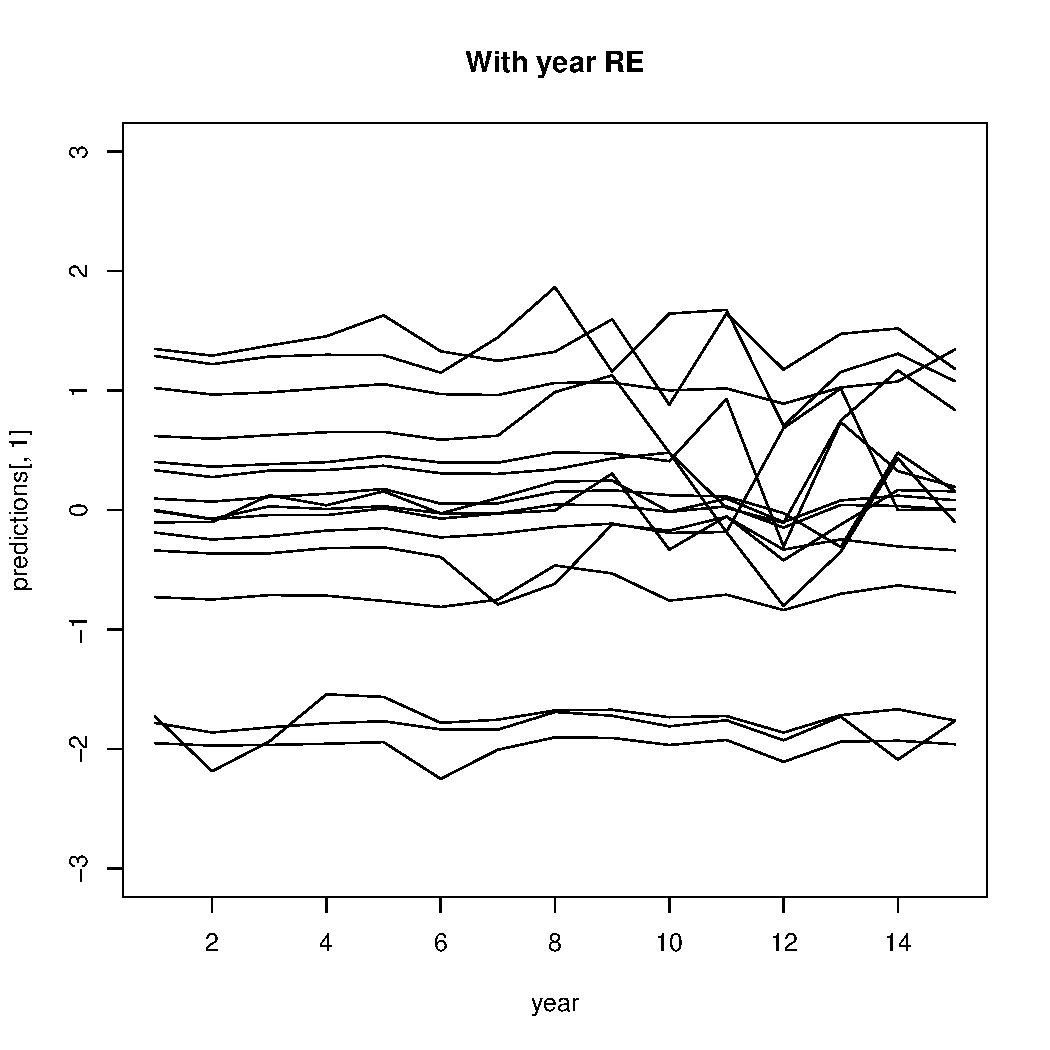
\includegraphics[width=\maxwidth]{figure/unnamed-chunk-20-1} 

\end{knitrout}

Intra-Class correlation:
\begin{knitrout}
\definecolor{shadecolor}{rgb}{0.969, 0.969, 0.969}\color{fgcolor}\begin{kframe}
\begin{alltt}
\hlstd{(cjs.interactionSdataNoS}\hlopt{$}\hlstd{BUGSoutput}\hlopt{$}\hlstd{mean}\hlopt{$}\hlstd{sigma.t}\hlopt{^}\hlnum{2}\hlstd{)}\hlopt{/}
  \hlstd{(cjs.interactionSdataNoS}\hlopt{$}\hlstd{BUGSoutput}\hlopt{$}\hlstd{mean}\hlopt{$}\hlstd{sigma.tXsp}\hlopt{^}\hlnum{2}\hlopt{+}
     \hlstd{cjs.interactionSdataNoS}\hlopt{$}\hlstd{BUGSoutput}\hlopt{$}\hlstd{mean}\hlopt{$}\hlstd{sigma.t}\hlopt{^}\hlnum{2}\hlstd{)}
\end{alltt}
\begin{verbatim}
## [1] 0.07141729
\end{verbatim}
\end{kframe}
\end{knitrout}

\begin{knitrout}
\definecolor{shadecolor}{rgb}{0.969, 0.969, 0.969}\color{fgcolor}\begin{kframe}
\begin{alltt}
\hlstd{iccpost} \hlkwb{<-} \hlkwd{vector}\hlstd{(}\hlkwc{length}\hlstd{=}\hlnum{1000}\hlstd{)}
\hlkwa{for} \hlstd{(ch} \hlkwa{in} \hlnum{1}\hlopt{:}\hlnum{1}\hlstd{)}
\hlstd{\{}
  \hlkwa{for} \hlstd{(itt} \hlkwa{in} \hlnum{1}\hlopt{:}\hlnum{1000}\hlstd{)}
  \hlstd{\{}
    \hlstd{iccpost[itt} \hlopt{+} \hlnum{1000}\hlopt{*}\hlstd{(ch}\hlopt{-}\hlnum{1}\hlstd{)]} \hlkwb{<-}
      \hlstd{cjs.interactionSdataNoS}\hlopt{$}\hlstd{BUGSoutput}\hlopt{$}\hlstd{sims.array[itt, ch,}\hlstr{"sigma.t"}\hlstd{]}\hlopt{^}\hlnum{2} \hlopt{/}
      \hlstd{( cjs.interactionSdataNoS}\hlopt{$}\hlstd{BUGSoutput}\hlopt{$}\hlstd{sims.array[itt, ch,}\hlstr{"sigma.t"}\hlstd{]}\hlopt{^}\hlnum{2} \hlopt{+}
          \hlstd{cjs.interactionSdataNoS}\hlopt{$}\hlstd{BUGSoutput}\hlopt{$}\hlstd{sims.array[itt, ch,}\hlstr{"sigma.tXsp"}\hlstd{]}\hlopt{^}\hlnum{2}\hlstd{)}
  \hlstd{\}}
\hlstd{\}}
\hlkwd{traceplot}\hlstd{(}\hlkwd{as.mcmc}\hlstd{(iccpost),} \hlkwc{ylim}\hlstd{=}\hlkwd{c}\hlstd{(}\hlnum{0}\hlstd{,}\hlnum{1}\hlstd{))}
\end{alltt}
\end{kframe}
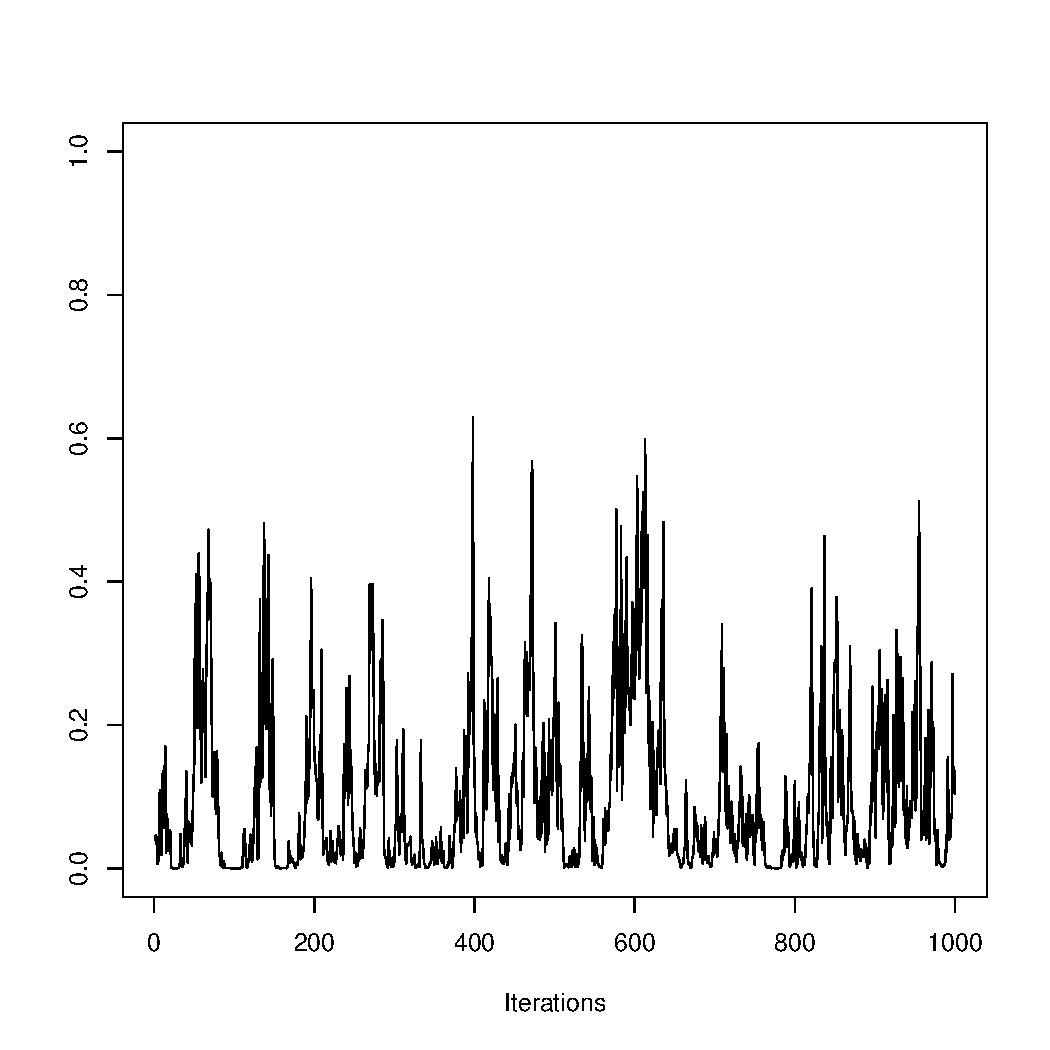
\includegraphics[width=\maxwidth]{figure/unnamed-chunk-22-1} 
\begin{kframe}\begin{alltt}
\hlkwd{plot}\hlstd{(}\hlkwd{density}\hlstd{(iccpost),} \hlkwc{xlim} \hlstd{=} \hlkwd{c}\hlstd{(}\hlnum{0}\hlstd{,}\hlnum{1}\hlstd{),}
     \hlkwc{main}\hlstd{=}\hlstr{"Synchrony estimate with no synchrony simulated"}\hlstd{)}
\end{alltt}
\end{kframe}
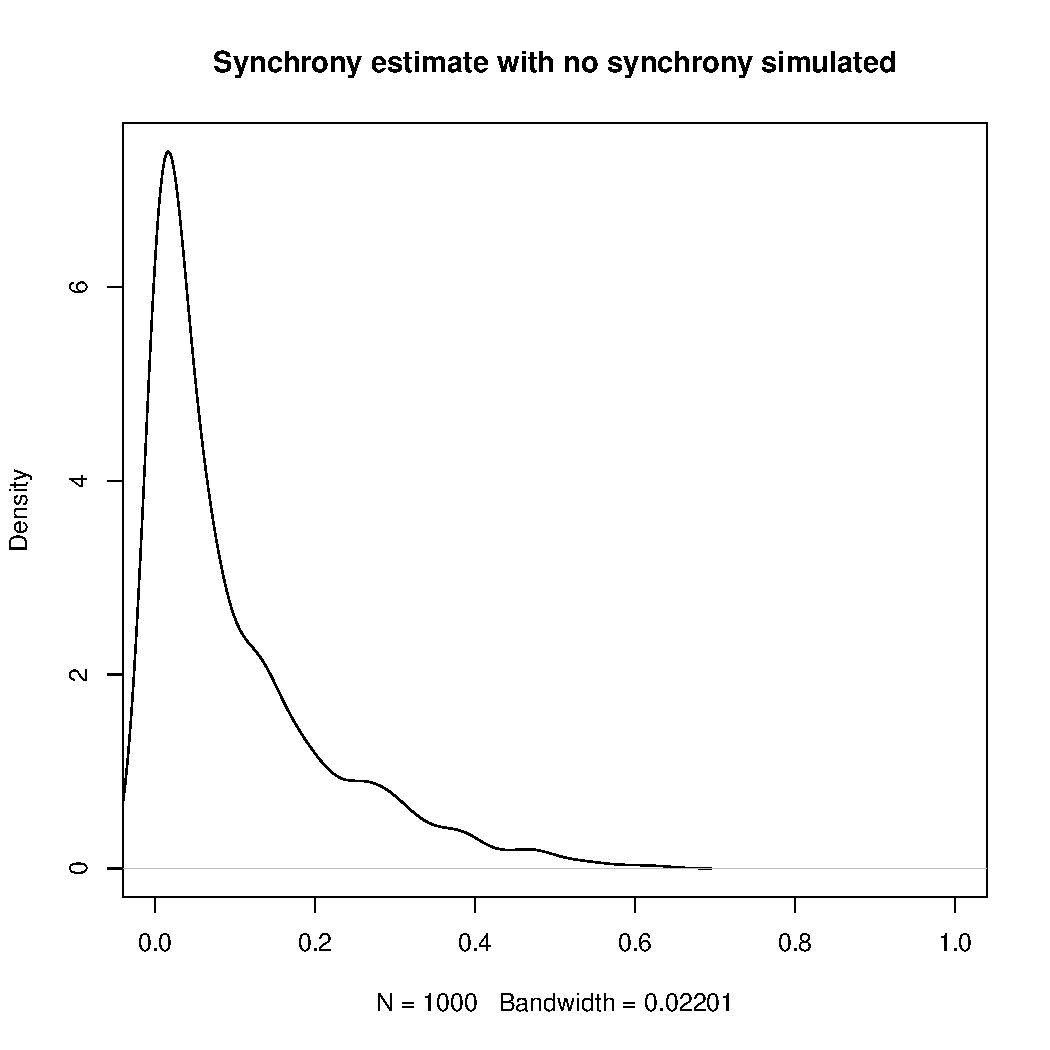
\includegraphics[width=\maxwidth]{figure/unnamed-chunk-22-2} 

\end{knitrout}
\end{document}
